
% TODO:
%   pow() function
%   .strip() string method
% memory diagrams -- diff between modifying in place and returning a copy (like
% .strip().)
% Left-side "variable names and atomic data". Right-side "aggregate data."

\chapter{Memory pictures and calculations}

Now that we've talked about the three important kinds of atomic variables,
let's consider the question of \textit{where they live}. It might sound like a
strange question. Aren't they ``in'' the Jupyter Notebook cell in which they
were typed?

Actually, no. And that brings me to the first mission-critical lesson of the
semester, which is a bane to all students who don't deeply learn it. The lesson
is:

\begin{quote}
\textbf{The code itself is only a means to an end. The purpose of the code is
to read or write what's in memory.}
\end{quote}

\textbf{Memory} is the part of the computer in which variables and their values
are stored. To use the terminology of Chapter~\ref{ch:atomicData}, memory is
where the environment lives. It is \textit{invisible} to the programmer, but it
is also \textit{very much there.} The single most important trick to learning
how to write correct code is being able to summon to mind what memory looks
like at any point in time. The code you must write is a natural consequence of
that.

\section{Memory pictures}

It's easier with pictures at first, so we'll draw plenty of them. Our
\textbf{memory pictures} will have a very specific format, and this is
crucially important: don't get creative with how things are labeled or where
things are drawn. In order for your code to work \textit{you must have this
picture exactly right.} It's not art; it's science.

Our memory pictures will always be divided into exactly two ``realms,'' one on
the left and one on the right, labeled as follows:

\begin{center}

\includegraphics[width=.7\textwidth]{memoryPicture.png}
\end{center}

The left column's name should be recognizable, since that's exactly what we
covered last chapter. The right column won't have anything in it until the next
chapter, so stay tuned.

\subsection{Writing to memory}

When we create atomic variables in a Code cell, a la:

\begin{Verbatim}[fontsize=\small,samepage=true,frame=single,framesep=3mm]
pin_count = 844
username = 'Bekka Palmer'
\end{Verbatim}

each one gets put on the left-hand side of the diagram as a \textbf{named box}.
The name of the box is the variable's name, and the thing inside of the box is
its value.

\vspace{-.2in}
\begin{center}
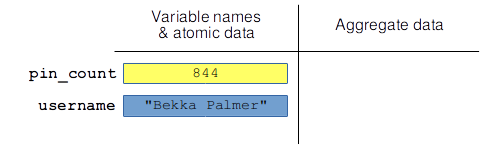
\includegraphics[width=.8\textwidth]{memoryPicture2.png}
\end{center}

It doesn't matter which boxes are higher or lower on the page, only that the
names stick with their boxes and don't get mixed up. As a bonus, I have colored
the boxes differently, indicating that \texttt{pin\_count} (an \texttt{int}) is
a different type than \texttt{username} (a \texttt{str}). \footnote{One other
tiny detail you might notice: even though our code had single quotes to delimit
Bekka Palmer's name, I put double quotes in the box in the memory picture. This
is to emphasize that no matter how you create a string in the code -- whether
with single quotes or double -- the underlying ``thing'' that gets written to
memory is the same. I'll always put double-quotes in memory pictures, just
because.}

Creating more variables just adds more named boxes:

\begin{Verbatim}[fontsize=\small,samepage=true,frame=single,framesep=3mm]
...
avg_num_impressions = 1739.3
board_name = "Things to Make"
\end{Verbatim}

\vspace{-.2in}
\begin{center}
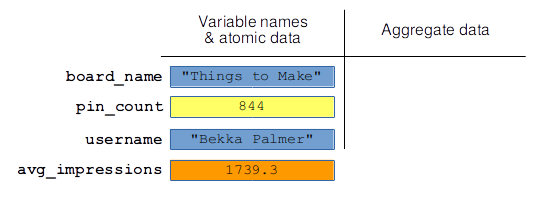
\includegraphics[width=.8\textwidth]{memoryPicture3.png}
\end{center}

I'm deliberately shuffling around the order of the boxes just to mess with you.
Python makes no guarantee of what ``order'' it will store variables in anyway,
and in reality it actually does become a big jumbled mess like this under the
hood. All Python guarantees is that it will consistently store a name, value,
and a type for each variable.

When we change the value of a variable (rather than creating a new one), the
value in the appropriate box gets updated:

\begin{Verbatim}[fontsize=\small,samepage=true,frame=single,framesep=3mm]
...
avg_num_impressions = 2000.97
pin_count = 845
another_board = 'Pink!'
\end{Verbatim}

\vspace{-.2in}
\begin{center}
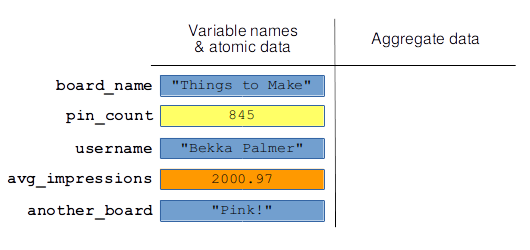
\includegraphics[width=.8\textwidth]{memoryPicture4.png}
\end{center}

Note carefully that \textit{the previous value in the box is completely
obliterated} and there is absolutely no way to ever get it back. There's no
way, in fact, to know that there even \textit{was} a previous value different
than the current one. Unless specifically orchestrated to do so, computer
programs only keep track of the present, not the past.
